\newcommand{\econtexRoot}{.}


\documentclass[10pt,english,t,10pt]{beamer}
\usepackage{lmodern}
\usepackage[T1]{fontenc}
\usepackage[utf8]{inputenc}
\setcounter{tocdepth}{1}
\setlength{\parskip}{\smallskipamount}
\setlength{\parindent}{0pt}
\usepackage{units}
\usepackage{amstext}
\usepackage{amssymb}
\usepackage{graphicx}
\usepackage[authoryear]{natbib}
\PassOptionsToPackage{normalem}{ulem}
\usepackage{ulem}

\usepackage{dcolumn}
\usepackage{verbatim}
\usepackage{cancel}
\usepackage{econtexShortcuts}
\usepackage{wasysym,ifthen,mathrsfs}
\usepackage[english]{babel}
\usepackage{color}
%\usepackage[latin1]{inputenc}
\usepackage{booktabs,natbib}
% Resources that need to be accessible from various different locations

\providecommand{\YLevBF}{\ensuremath{\mathbf{Y}}}
\renewcommand{\pDies}{\ensuremath{\mathsf{d}}}
%\renewcommand{\PDies}{\ensuremath{\mathsf{D}}}
%\renewcommand{\PLives}{\ensuremath{(1-\mathsf{D})}}

\providecommand{\aggrSavingRuleCoeff}{\ensuremath{\kappa}}
\providecommand{\stnRatio}{\ensuremath{\tau}}

\newcommand{\TabsDir}{\econtexRoot/Tables}\newcommand{\Calibration}{\econtexRoot/Calibration}
\newcommand{\W}{\mathcal{W}}            % Include or exclude aggregate wage in individual problem - to include, should be \newcommand{\W}{W}

\provideboolean{Depreciation}
\setboolean{Depreciation}{true}
%\setboolean{Depreciation}{false}
\provideboolean{MicroDepr}
\setboolean{MicroDepr}{true}
%\setboolean{Depreciation}{false}
\newcommand{\ifDepr}{\ifthenelse{\boolean{Depreciation}}}
\newcommand{\MicroDepr}{\ifthenelse{\boolean{MicroDepr}}}

\newcommand{\RBet}{\mathbf{R}} % Bold  version is between-period rate; \mathcal version is within
\newcommand{\rBet}{\mathbf{r}} % Bold  version is between-period rate; \mathcal version is within
\newcommand{\RIn}{\mathcal{R}}
\newcommand{\rIn}{r}


\provideboolean{Growth}
\setboolean{Growth}{true}
\setboolean{Growth}{false}
\newcommand{\ifGG}{\ifthenelse{\boolean{Growth}}}  % Switch for whether to include productivity growth in formulae; useful for programming/debugging

\provideboolean{numSwitch}     % Switch that suppresses eqn numbers on slides but not in text
\setboolean{numSwitch}{true}   % Set to true  at beginning of text
%\setboolean{numSwitch}{false} % Set to false at beginning of slides
\providecommand{\ifnumSw}{\ifthenelse{\boolean{numSwitch}}{}{\nonumber}}

\provideboolean{Slides}
\setboolean{Slides}{false}
\newcommand{\ifslides}{\ifthenelse{\boolean{Slides}}}

\provideboolean{ZeroProb}
\setboolean{ZeroProb}{false}
\setboolean{ZeroProb}{true}
\newcommand{\ifZero}{\ifthenelse{\boolean{ZeroProb}}}

\provideboolean{DocVersion} % If true, produce an elaborate version of the document that contains all formulae used in the software
\setboolean{DocVersion}{false}
\setboolean{DocVersion}{true}
%\providecommand{\ifDoc}{\ifthenelse{\boolean{DocVersion}}}
\providecommand{\ifDoc}{\marginpar{\tiny{DocAndNodocVersions}}\emph}

% ExtraExplain toggles whether to include the explanation for why we can't assume \bar{\ell}=\ell
\provideboolean{ExtraExplain}
\setboolean{ExtraExplain}{false}
%\setboolean{ExtraExplain}{true}
\newcommand{\ifExplain}{\ifthenelse{\boolean{ExtraExplain}}}

\provideboolean{ShowStickyE}
\setboolean{ShowStickyE}{true}
\setboolean{ShowStickyE}{false}
\newcommand{\StickyE}{\ifthenelse{\boolean{ShowStickyE}}}

\newcommand{\eq}{\econtexRoot/Equations}
\newcommand{\EqnDir}{\econtexRoot/Equations}

\newcommand{\fm}{frictionless-$\mathbf{m}$ }
\newcommand{\sm}{sticky-$\mathbf{m}$ }

\newcommand{\ParmDir}{\econtexRoot/Calibration}
\newcommand{\TablesDir}{\econtexRoot/Tables}
\newcommand{\DirCampManVsStickyE}{\econtexRoot/Empirical/US/Results/LaTeX/tables}
\providecommand{\perc}[1]{\widetilde{#1}}



\makeatletter
%%%%%%%%%%%%%%%%%%%%%%%%%%%%%% Textclass specific LaTeX commands.
% this default might be overridden by plain title style
\newcommand\makebeamertitle{\frame{\maketitle}}%
% (ERT) argument for the TOC
\AtBeginDocument{%
	\let\origtableofcontents=\tableofcontents
	\def\tableofcontents{\@ifnextchar[{\origtableofcontents}{\gobbletableofcontents}}
	\def\gobbletableofcontents#1{\origtableofcontents}
}

%%%%%%%%%%%%%%%%%%%%%%%%%%%%%% User specified LaTeX commands.

\definecolor{mygray}{gray}{0.6}

\usepackage{tikz}
\usetikzlibrary{positioning}
\usepackage{appendixnumberbeamer}

\usepackage{graphicx}
\usepackage{subfig}

\usetheme[progressbar=frametitle,block=fill,subsectionpage=progressbar]{metropolis}

% margin
\setbeamersize{text margin right=1.5cm}

% colors
\colorlet{DarkRed}{red!70!black}
\setbeamercolor{normal text}{fg=black}
\setbeamercolor{alerted text}{fg=DarkRed}
\setbeamercolor{progress bar}{fg=DarkRed}
\setbeamercolor{button}{bg=DarkRed}

% width of seperators
\makeatletter
\setlength{\metropolis@titleseparator@linewidth}{1pt}
\setlength{\metropolis@progressonsectionpage@linewidth}{1pt}
\setlength{\metropolis@progressinheadfoot@linewidth}{1pt}
\makeatother

% new alert block
\newlength\origleftmargini
\setlength\origleftmargini\leftmargini
\setbeamertemplate{itemize/enumerate body begin}{\setlength{\leftmargini}{4mm}}
\let\oldalertblock\alertblock
\let\oldendalertblock\endalertblock
\def\alertblock{\begingroup \setbeamertemplate{itemize/enumerate body begin}{\setlength{\leftmargini}{\origleftmargini}} \oldalertblock}
\def\endalertblock{\oldendalertblock \endgroup}
\setbeamertemplate{mini frame}{}
\setbeamertemplate{mini frame in current section}{}
\setbeamertemplate{mini frame in current subsection}{}
\setbeamercolor{section in head/foot}{fg=normal text.bg, bg=structure.fg}
\setbeamercolor{subsection in head/foot}{fg=normal text.bg, bg=structure.fg}

% footer
\makeatletter
\setbeamertemplate{footline}{%
	\begin{beamercolorbox}[colsep=1.5pt]{upper separation line head}
	\end{beamercolorbox}
	\begin{beamercolorbox}{section in head/foot}
		\vskip1pt\insertsectionnavigationhorizontal{\paperwidth}{}{\hskip0pt plus1filll \insertframenumber{} / \inserttotalframenumber \hskip2pt}\vskip3pt% 
	\end{beamercolorbox}%
	\begin{beamercolorbox}[colsep=1.5pt]{lower separation line head}
	\end{beamercolorbox}
}
\makeatother

% toc
\setbeamertemplate{section in toc}{\hspace*{1em}\inserttocsectionnumber.~\inserttocsection\par}
\setbeamertemplate{subsection in toc}{\hspace*{2em}\inserttocsectionnumber.\inserttocsubsectionnumber.~\inserttocsubsection\par}


% Automatically create vspace between items
% See: https://tex.stackexchange.com/questions/369504/beamer-vertically-stretching-level-1-list-items-in-a-nested-list-environment
%\usepackage{xpatch} 
%\xpatchcmd{\itemize}   
%	{\def\makelabel}   
%	{\ifnum\@itemdepth=1\relax      
%		\setlength\itemsep{\fill} % separation for first level    
%		\fi\def\makelabel   
%	}{}{} 
%\xpatchcmd{\enditemize}   
%	{\endlist}   
%	{\endlist\ifnum\@itemdepth<2\else\vfil\fi}{}{}




% Automatically create vspace between items
% See: https://jayrobwilliams.com/posts/2019/10/better-beamer
\makeatletter
\renewcommand{\itemize}[1][]{%
	\beamer@ifempty{#1}{}{\def\beamer@defaultospec{#1}}%
	\ifnum \@itemdepth >2\relax\@toodeep\else
	\advance\@itemdepth\@ne
	\beamer@computepref\@itemdepth% sets \beameritemnestingprefix
	\usebeamerfont{itemize/enumerate \beameritemnestingprefix body}%
	\usebeamercolor[fg]{itemize/enumerate \beameritemnestingprefix body}%
	\usebeamertemplate{itemize/enumerate \beameritemnestingprefix body begin}%
	\list
	{\usebeamertemplate{itemize \beameritemnestingprefix item}}
	{\def\makelabel##1{%
			{%
				\hss\llap{{%
						\usebeamerfont*{itemize \beameritemnestingprefix item}%
						\usebeamercolor[fg]{itemize \beameritemnestingprefix item}##1}}%
			}%
		}%
	}
	\fi%
	\setlength\itemsep{\fill}
	\ifnum \@itemdepth >1
	\vfill
	\fi%  
	\beamer@cramped%
	\raggedright%
	\beamer@firstlineitemizeunskip%
}

\def\enditemize{\ifhmode\unskip\fi\endlist%
	\usebeamertemplate{itemize/enumerate \beameritemnestingprefix body end}
	\ifnum \@itemdepth >1
	\vfil
	\fi%  
}
\makeatother

\makeatother





%%% Jirka's colors

\definecolor{myRed}{rgb}{0.8,0,0}
\definecolor{jirkasblue}{rgb}{0.2,0.2,0.7}
\definecolor{jirkasred}{rgb}{0.9,0,0}
\definecolor{LightCyan}{rgb}{0.88,1,1}
\definecolor{SlideNavy}{rgb}{0,0,0.54}
\definecolor{StataDarkBlue}{rgb}{0,0,0.835}
\definecolor{Pink}{rgb}{1,0.8,0.8}

\newcolumntype{g}{>{\columncolor{Pink}}d{3}}
\newcommand{\jemph}[1]{{\color{StataDarkBlue}#1}}
\newcommand{\jbemph}[1]{\textbf{\color{SlideNavy}#1}}
\newcommand{\var}{\ensuremath{\text{var}}}

%%%%%%%%%%%%%%%  Beamer setup
%%%%%%%%%%%%%%%%%%%%%%%%%%%%%%%%%%%%%%%%%%%%%%%%%%%%%%%%%%%%%%%%%%%%%%%%%%%%%%%%%%%%%%%%%%%%%%%%%%%%%%%%%%%%%%
%\mode<presentation>
%{
%  \usetheme{Warsaw} % Singapore % Montpellier
%  \setbeamercovered{transparent}
%}
%
%% if this is on, bullets are shown step by step
%\beamerdefaultoverlayspecification{<+->}

%\setbeamertemplate{navigation symbols}{}  % Take away navigation symbols


%%%%%%%%%%%%%%%  Chris's definitions
%%%%%%%%%%%%%%%%%%%%%%%%%%%%%%%%%%%%%%%%%%%%%%%%%%%%%%%%%%%%%%%%%%%%%%%%%%%%%%%%%%%%%%%%%%%%%%%%%%%%%%%%%%%%%%

\providecommand{\W}{\mathcal{W}}            % Include or exclude aggregate wage in individual problem - to include, should be
\providecommand{\perc}[1]{\widetilde{#1}}

\provideboolean{Depreciation}
\setboolean{Depreciation}{true}
%\setboolean{Depreciation}{false}
\provideboolean{MicroDepr}
\setboolean{MicroDepr}{true}
% \setboolean{Depreciation}{false}


\newboolean{includeTF}
\setboolean{includeTF}{true}

\newcommand{\ifInclude}[1]{\ifthenelse{\boolean{includeTF}}{#1}}
\providecommand{\ifDepr}{\ifthenelse{\boolean{Depreciation}}}
\providecommand{\MicroDepr}{\ifthenelse{\boolean{MicroDepr}}}

\ifDepr{
	\providecommand{\RBet}{\mathbf{R}} % Bold  version is between-period rate; \mathcal version is within
	\providecommand{\rBet}{\mathbf{r}} % Bold  version is between-period rate; \mathcal version is within
	\providecommand{\RIn}{\mathcal{R}}
	\providecommand{\rIn}{r}
}{
	\providecommand{\RBet}{R} % Bold  version is between-period rate; \mathcal version is within
	\providecommand{\rBet}{r} % Bold  version is between-period rate; \mathcal version is within
	\providecommand{\RIn}{R}
	\providecommand{\rIn}{r}
	\providecommand{\rNet}{\mathfrak{r}} % For defining consumption Euler equation
}


\provideboolean{Growth}
\setboolean{Growth}{true}
\setboolean{Growth}{false}
\providecommand{\ifGG}{\ifthenelse{\boolean{Growth}}}  % Switch for whether to include productivity growth in formulae; useful for programming/debugging

\provideboolean{numSwitch}     % Switch that suppresses eqn numbers on slides but not in text
\setboolean{numSwitch}{true}   % Set to true  at beginning of text
%\setboolean{numSwitch}{false} % Set to false at beginning of slides
\providecommand{\ifnumSw}{\ifthenelse{\boolean{numSwitch}}{}{\nonumber}}

\provideboolean{Slides}
\setboolean{Slides}{false}
\providecommand{\ifslides}{\ifthenelse{\boolean{Slides}}}

\provideboolean{ZeroProb}
\setboolean{ZeroProb}{false}
\setboolean{ZeroProb}{true}
\providecommand{\ifZero}{\ifthenelse{\boolean{ZeroProb}}}

\provideboolean{DocVersion} % If true, produce an elaborate version of the document that contains all formulae used in the software
\setboolean{DocVersion}{false}
\setboolean{DocVersion}{true}
\providecommand{\ifDoc}{\ifthenelse{\boolean{DocVersion}}}

% ExtraExplain toggles whether to include the explanation for why we can't assume \bar{\ell}=\ell
\provideboolean{ExtraExplain}
\setboolean{ExtraExplain}{true}
\providecommand{\ifExplain}{\ifthenelse{\boolean{ExtraExplain}}}

\provideboolean{ShowStickyE}
\setboolean{ShowStickyE}{true}
\setboolean{ShowStickyE}{false}
\providecommand{\StickyE}{\ifthenelse{\boolean{ShowStickyE}}}

\provideboolean{BoE}
\setboolean{BoE}{true}
\setboolean{BoE}{false}
\providecommand{\BoEYN}{\ifthenelse{\boolean{BoE}}}

\providecommand{\BoEHideBegin}{\ifthenelse{\boolean{BoE}}{\setboolean{includeTF}{false}}{}}
\providecommand{\BoEHideEnd}{  \ifthenelse{\boolean{BoE}}{\setboolean{includeTF}{true}}{}}

\providecommand{\TimeShortHideBegin}{\ifthenelse{\boolean{TimeShort}}{\setboolean{includeTF}{false}}{}}
\providecommand{\TimeShortHideEnd}{  \ifthenelse{\boolean{TimeShort}}{\setboolean{includeTF}{true}}{}}


\provideboolean{TimeShort}
\setboolean{TimeShort}{true}
%\setboolean{TimeShort}{false}
\providecommand{\TimeShortYN}{\ifthenelse{\boolean{TimeShort}}}


\providecommand{\econtexRoot}{.}
\providecommand{\eq}{\econtexRoot/Equations}

\providecommand{\fm}{frictionless-$\mathbf{m}$ }
\providecommand{\sm}{sticky-$\mathbf{m}$ }

\providecommand{\ParmDir}{\econtexRoot/Calibration/Parameters}
\providecommand{\TablesDir}{\TabsDir}
%\providecommand{\ParmDir}{C:/Jirka/Research/stickyConsumptionUS/Nov26_07/cAndCwithStickyEArchive/Calibration/Parameters}
%\providecommand{\TablesDir}{C:/Jirka/Research/stickyConsumptionUS/Nov26_07/cAndCwithStickyEArchive/Tables}

\definecolor{jirkasred}{rgb}{0.9,0,0}
\definecolor{jirkasblue}{rgb}{0.2,0.2,0.7}
\providecommand{\jemph}[1]{{\color{jirkasblue}#1}}
\def\newblock{\hskip .11em plus .33em minus .07em}


\newcolumntype{d}[1]{D{.}{.}{#1}}

%\usepackage[latin1]{inputenc}

% END OF CARROLL STUFF

\usepackage{babel}
\begin{document}
	\title{3. Consumption-Saving Models: Extensions \vspace{-2mm}}
	\subtitle{Adv. Macro: Heterogenous Agent Models} 
	\author{Jeppe Druedahl \& Patrick Moran}
	\date{2022}
	
	{
		\setbeamertemplate{footline}{} 
		\begin{frame}
		
		\maketitle
		
		\begin{tikzpicture}[overlay, remember picture]
		\node[above left=0cm and 0.0cm of current page.south east] 
		{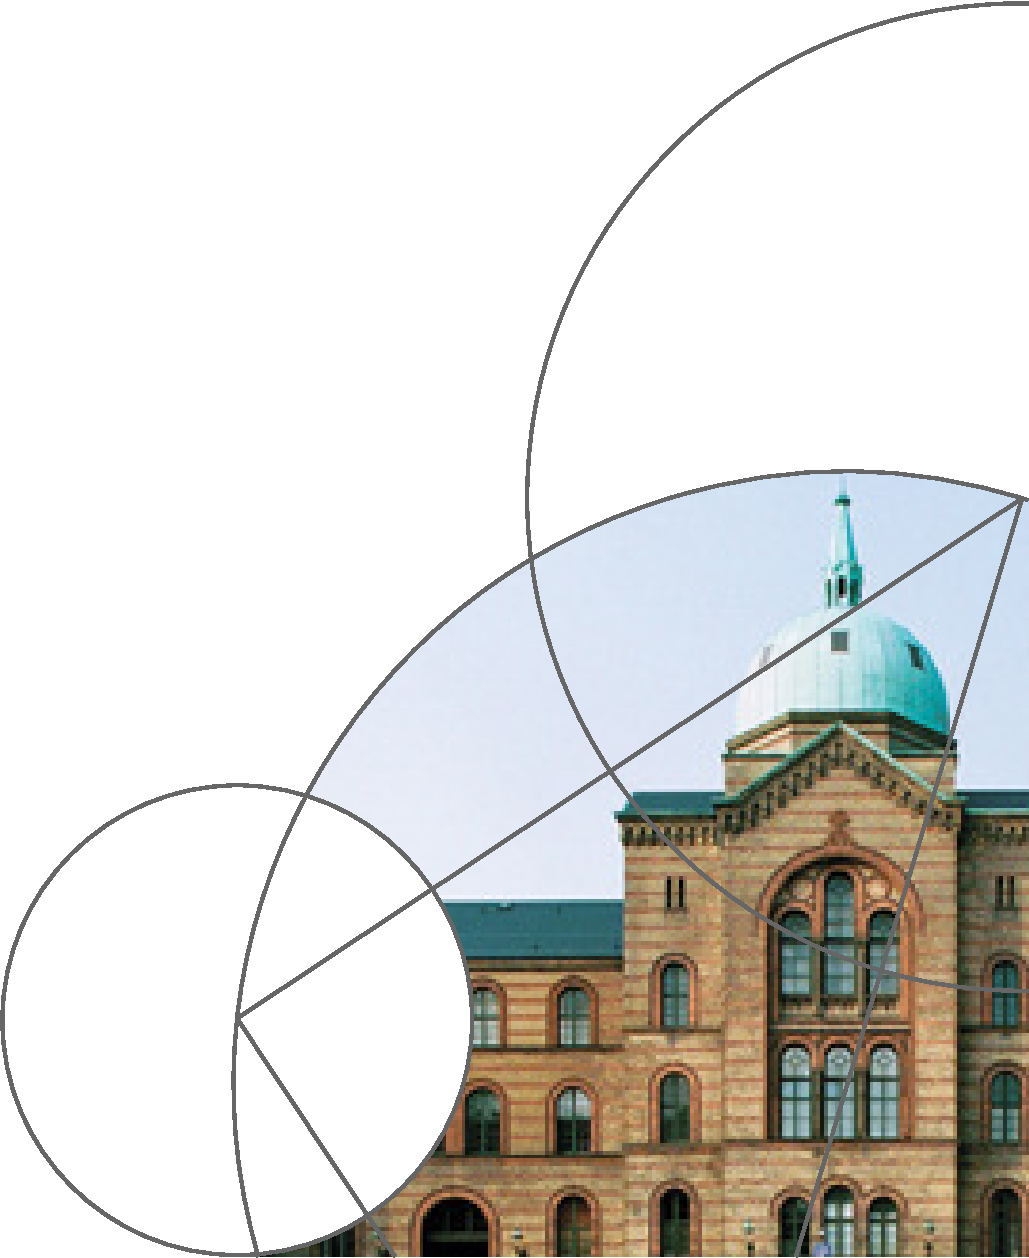
\includegraphics[width=4cm]{../figs/KUSAMFtitlelrcorner.pdf}};
		\end{tikzpicture}
		
		\begin{tikzpicture}[overlay, remember picture]
		\node[below left=0.5cm and .8cm of current page.north east] 
		{\includegraphics[width=1.5cm]{../figs/KUSAMFlogo.pdf}};
		\end{tikzpicture}
		
		\begin{tikzpicture}[overlay, remember picture]
		\node[below right=0.5cm and 0.8cm of current page.north west] 
		{
\includegraphics[width=1.5cm]{../figs/CEBI.png}};
		\end{tikzpicture}
		
		\begin{tikzpicture}[overlay, remember picture]
		\node[above right=0.5cm and 0.8cm of current page.south west] 
		{
\includegraphics[width=1.5cm]{../figs/DNRF.png}};
		\end{tikzpicture}
		
	\end{frame}
}

\addtocounter{framenumber}{-1}


\section{Introduction}
\begin{frame}{Disclaimer}
\vspace{-2mm}

\vspace{20mm}
\begin{itemize}
	\item Note: The views expressed in this presentation are those of the author
	and do not represent the views of the Federal Reserve Board or Federal
	Reserve System.
\end{itemize}
\end{frame}


\newcolumntype{d}[1]{D{.}{.}{#1}}
\def\newblock{\hskip .11em plus .33em minus .07em}




\begin{frame}{Consumption-Saving Models}
\vspace{-2mm}
\begin{itemize}
	\item <+->\textbf{Goal for today: }Extend the traditional consumption-saving
	model to better capture important aspects of household behavior 
	\item <+->\textbf{Central economic questions:}
	\begin{enumerate}
		\item How do we explain excess smoothness in consumption data?
		\item How to distinguish between habits vs inattention?
		\item What if households have trouble saving due to temptation? \vfill
	\end{enumerate}
	\item <+->\textbf{Plan for today:}
	\begin{enumerate}
		\item Discuss the problem of ``excess smoothness'' of consumption
		\item Study the model of sticky expectations (Carroll et al,
		2019)
		\item Study the model of temptation and commitment (Attanasio
		et al, 2021)
	\end{enumerate}
\end{itemize}
\end{frame}
%

% \section{Consumption Habits}
\section{Excess Smoothness}
\begin{frame}{Excess smoothness}

	\begin{itemize}       
		
		\item  One of the key puzzles in consumption-saving models is the ``excess smoothness'' of consumption
	
	\begin{itemize}       
		
		\item  Theory:  Consumption responds instantly, completely to shock           
%			\item Consequences of uncertainty are trivial        
		

		
		\item Evidence: Consumption is too smooth 
	
%		\item Solution: \jbemph{``Habits'' parameter $\chi^{\text{Macro}}\approx 0.6\sim~0.8$}\\ \centerline{       $\Delta \log \mathbf{C}_{t+1} = \varsigma + \chi \Delta \log \mathbf{C}_t +\epsilon $}       
	\end{itemize}     

\pause

		\item Campbell and Deaton (1989): Consumption does not react sufficiently to innovations to the permanent component of income
	
	\end{itemize}     

\end{frame}




\begin{frame}
\frametitle{Theory: Simple Model with Quadratic Utility }

\begin{block}{\cite{hallRandomWalk} Random Walk}
%	\phantom{.}
	\begin{itemize}
		\item Household utility 
		\[
		\mathbb{E}_{0}\sum_{t=0}^{\infty}\beta^{t}\uFunc(\cLevBF_{t})
		\]
		
		\pause
		\item \jemph{Total Wealth} (Human$\,+\,$Nonhuman):\\
		\begin{center}
			{$\wAllLev_{t+1} = (\wAllLev_{t}-\cLevBF_{t})\Rfree+\zeta_{t+1}$}
		\end{center}\vfill
	\pause
	
		\item \jemph{C Euler Equation}: \\
		\begin{center}
			{$\uFunc^{\prime}(\cLevBF_{t}) = \Rfree\beta \Ex_{t}[\uFunc^{\prime}(\cLevBF_{t+1})]$}
		\end{center}\vfill
	\pause
	\item For simplicity, assume quadratic utility ($\uFunc(c) = c^2$) and $\Rfree\beta=1$ \vfill
	\pause
		\item Under these assumptions, consumption follows a \jemph{random walk}: \\
		\begin{center}
			{$\Delta \cLevBF_{t+1} = \epsilon_{t+1}$}
		\end{center}
	\end{itemize}
\end{block}

\pause
But in the data: permanent income much nosier than consumption

\end{frame}



\subsection{One Explanation: Habit Formation}
\begin{frame}{Popular solution in DSGE models: habit formation}

\begin{itemize}
\item <+->Household utility depends on both $c_{i, t}$ and $c_{i, t-1}$
\[
\mathbb{E}_{0}\sum_{t=0}^{\infty}\beta^{t}u(\tilde{c}_{i,t})
\]
\item where 
\[
\tilde{c}_{i,t}=c_{i,t}-\chi c_{i,t-1}
\]
\vfill\vfill
\item $\chi$ is positive if goods provide services across periods 
%\item negative if goods are addictive (habit formation), 
\item zero if goods are fully non-durable, non-habit forming
\end{itemize}

\end{frame}





\begin{frame}{Testable implications of habit formation}

\begin{itemize}
	\item Consumption Euler equation (for full derivation, see Dynan 2000):
	\[
	E_t\left[(1+r) \beta \frac{MU_{i, t+1}}{MU_{i, t}}\right]=1
	\]
	\vfill 
	
	\pause
	\item If we assume CRRA utility function, $u(c) = \frac{c^{1-\rho}}{1-\rho}$ then:
	\[
	(1+r) \beta \left(\frac{\tilde{c}_{i, t}}{\tilde{c}_{i, t-1}}\right)^{-\rho}=1+\varepsilon_{i, t} 
	\]
	where $\varepsilon_{i, t} $ is the expectational error \vfill 
	

	
\end{itemize}

\end{frame}




\begin{frame}{Testable implications of habit formation}

\begin{itemize}
 
	\item Taking logs and substituting for $\tilde{c}$ gives:
	\[ 
	\Delta \ln \left(c_{i, t}-\chi c_{i, t-1}\right) 
	= \frac{1}{\rho}[\ln (1+r)+\ln (\beta)] -\frac{1}{\rho} \ln \left(1+\varepsilon_{i, t}\right) 
	\]
	\vfill 
	
	\pause
	\item This yields the following estimable equation:
	\[
	\Delta \ln \left(c_{i, t}\right)= \gamma_0+\chi \Delta \ln \left(c_{i, t-1}\right) +e_{i, t}
	\]
	which can be estimated on either micro data or macro data \\ (if macro data, then just remove the $i$ subscript)
	\vfill 
	


	
\end{itemize}

\end{frame}



\begin{frame}
\frametitle{Empirical estimates of habit persistence}

\begin{itemize}
	\item $\chi$ has been estimated by over 597 different papers
	\begin{figure}
		\begin{center}
			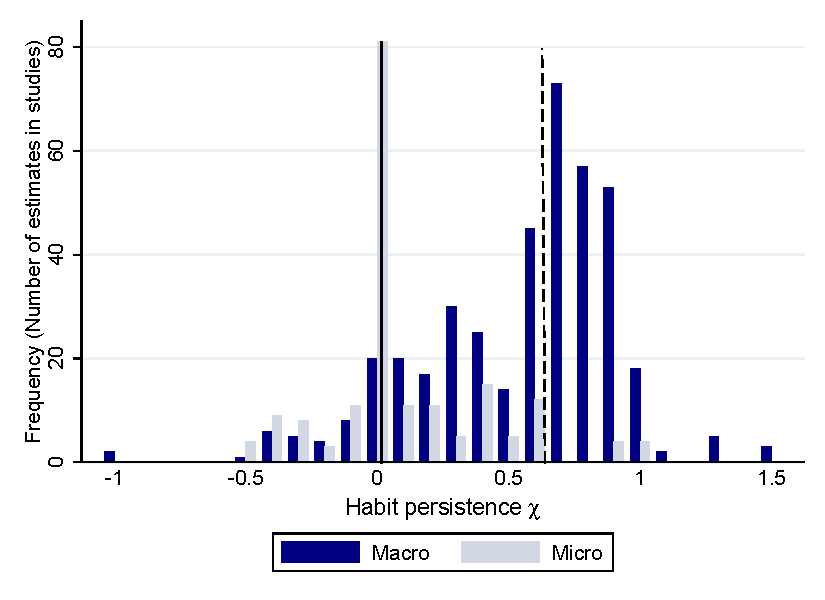
\includegraphics[width=.75\textwidth]{../Figures/microMacroMetaHistogram}
		\end{center}
	\end{figure}
	\item  Mean $\chi$ in macro studies: 0.6
	\item Mean $\chi$ in micro studies: 0.0-0.1 
\end{itemize}

\end{frame}

\begin{frame}
\frametitle{Why the disagreement between macro and micro studies?}

\begin{block}{Macro: Representative Agent Models}
	\begin{itemize}
		\item  Theory: C responds instantly, completely to shock
		\item Evidence: Consumption is too smooth {\scriptsize (Campbell {\&} Deaton, 1989)}
		\item Solution: \jbemph{``Habits'' parameter $\chi^{\text{Macro}}\approx 0.6\sim~0.8$}\\
%		\centerline{       $\Delta \log \mathbf{C}_{t+1} = \varsigma + \chi \Delta \log \mathbf{C}_t +\epsilon $}
	\end{itemize}
\end{block}

\pause 

\begin{block}{Micro: Heterogeneous Agent Models}
	\begin{itemize}
		\item  \jbemph{Uninsurable risk is essential, changes everything}
		\item Var of micro income shocks much larger than of macro shocks:\\
		\centerline{    \jemph{var$(\Delta \log \pLevBF) \approx  100\times$var($\Delta \log \PLevBF$)}}
		\item Evidence: \jbemph{``Habits'' parameter $\chi^{\text{Micro}}\approx 0.0\sim 0.1$}
	\end{itemize}
\end{block}

\end{frame}





% Carroll et al 2019

\section{Macro Inattention}
%\subsection{Inattention}
\begin{frame}
\frametitle{Alternative Explanation: Inattention to Macro Aggregates}
\jbemph{Carroll, Crawley, Slacalek, Tokuoka, White (2019):}
\begin{itemize}
\item   Income Has Idiosyncratic and Aggregate Components
\item   Idiosyncratic Component Is Perfectly Observed
\item   Aggregate Component Is Stochastically Observed
\end{itemize}

\vfill 
%\jbemph{Is this theory plausible?}
%
%\begin{block}{\textbf{Idiosyncratic Variability Is $\sim$ 100$\times$ Bigger}}
%	\begin{itemize}
%		\item  If Same Specification Estimated on Micro vs Macro Data
%		\item  Pervasive Lesson of All Micro Data
%	\end{itemize}
%\end{block}
%
%\begin{block}{\textbf{Utility Cost of Inattention Small}}
%	\begin{itemize}
%		\item  Micro: Critical (and Easy) To Notice You're Unemployed
%		% \item Unlike \cite{pischkeMicroMacro}
%		\item  Macro: {\it Not} Critical To {\it Instantly} Notice If U $\uparrow$
%	\end{itemize}
%\end{block}

\pause

\begin{block}{\textbf{Idiosyncratic Variability Is $\sim$ 100$\times$ Bigger}}
\begin{itemize}
\item  If Same Specification Estimated on Micro vs Macro Data
\item  Pervasive Lesson of Micro Data
\end{itemize}
\end{block}

\pause

\begin{block}{\textbf{Utility Cost of Inattention Small}}
\begin{itemize}
\item  Micro: Critical (and Easy) To Notice You're Unemployed

\item  Macro: {\it Not} Critical To {\it Instantly} Notice If U $\uparrow$
\end{itemize}
\end{block}
\end{frame}

\TimeShortHideBegin








%\section{\href{http://www.econ2.jhu.edu/people/ccarroll/public/LectureNotes/Consumption/StickyExpectationsC/}{Toy Model}}
%\subsection{Toy Model}
\begin{frame}
\frametitle{Returning to simple theory}

\begin{block}{\cite{hallRandomWalk} Random Walk}
\phantom{.}
\begin{itemize}
\item \jemph{Total Wealth} (Human$\,+\,$Nonhuman):\\
\begin{center}
{$\wAllLev_{t+1} = (\wAllLev_{t}-\cLevBF_{t})\Rfree+\zeta_{t+1}$}
\end{center}
\item \jemph{C Euler Equation}: \\
\begin{center}
{$\uFunc^{\prime}(\cLevBF_{t}) = \Rfree\beta \Ex_{t}[\uFunc^{\prime}(\cLevBF_{t+1})]$}
\end{center}
\item $\Rightarrow$ \jemph{Random Walk} (for $\Rfree\beta=1$): \\
\begin{center}
{$\Delta \cLevBF_{t+1} = \epsilon_{t+1}$}
\end{center}
\item \jemph{Expected Wealth}: \\
\begin{center}
{$\wAllLev_{t} = \Ex_{t}[\wAllLev_{t+1}] = \Ex_{t}[\wAllLev_{t+2}] = \dots$}
\end{center}
\end{itemize}
\end{block}

\end{frame}


\begin{frame}
\frametitle{Sticky Expectations---Individual $\mathbf{c}$}

\begin{itemize}
\item
Consumer who happens to update at $t$ and $t+n$
\begin{eqnarray*}
\ifnumSw         \cLevBF_{t  } & = & (\rfree/\Rfree)\wAllLev_{t} \label{eq:ct}
\pause
\ifnumSw \\      \cLevBF_{t+1} & = & (\rfree/\Rfree)\perc{\wAllLev}_{t+1} = (\rfree/\Rfree)     \wAllLev _{t} = \cLevBF_{t}
\pause
%\ifnumSw \\      \cLevBF_{t+2} & = & (\rfree/\Rfree)\perc{\wAllLev}_{t+2} = (\rfree/\Rfree)     \wAllLev _{t} = \cLevBF_{t}
\ifnumSw \\               \vdots  &  & \vdots \nonumber
\ifnumSw \\        \cLevBF_{t+n-1} & = & \cLevBF_{t}
\label{eq:ctpn}
\end{eqnarray*}

\pause
\item
Implies that $\Delta^{n} \wAllLev_{t+n} \equiv \wAllLev_{t+n}-\wAllLev_{t}$ is white noise

\pause
\item So \jbemph{individual} $\mathbf{c}$ is RW across updating periods:
\begin{eqnarray*}
\ifnumSw  \mathbf{c}_{t+n}-\mathbf{c}_{t} & = & (\rfree/\Rfree)\underbrace{(\wAllLev_{t+n}-\wAllLev_{t}) }_{\Delta^{n} \wAllLev_{t+n}}
\end{eqnarray*}
%\item \jbemph{No persistence in individual c growth}
\end{itemize}
\end{frame}

\begin{frame}
\frametitle{Sticky Expectations---Aggregate $\mathbf{C}$}

\begin{itemize}
\setlength{\itemsep}{2mm}
\item Population normed to one, uniformly dist on $[0,1]$:
$\CLevBF_{t} = \int_{0}^{1} \cLevBF_{t,i}\,\text{d}i$

\pause
\item \jbemph{Calvo-Type Updating of Expectations:}
(Probability $\Pi = 0.25$, per quarter)

\pause
\item Economy composed of many sticky-$\Ex$ consumers:
\begin{eqnarray*}
 \CLevBF_{t+1} & = & (1-\Pi) \underbrace{\CLevBF^{\cancel{{\pi}}}_{t+1}}_{=\CLevBF_{t}} \label{eq:Ctp1} + \Pi \CLevBF^{{\pi}}_{t+1}
 \\
%\end{eqnarray*}
%\begin{eqnarray*}
  \Delta \mathbf{C}_{t+1} & \approx & \underbrace{(1-\Pi)}_{{}\equiv\chi=0.75} \Delta \mathbf{C}_{t} + \epsilon_{t+1}
\end{eqnarray*}
\pause
\item \jbemph{Substantial persistence ($\chi=0.75$) in aggregate C growth}
\end{itemize}
\end{frame}


\begin{frame}
\frametitle{One More Ingredient: Idiosyncratic Uncertainty \dots}

\begin{itemize}
\setlength{\itemsep}{3mm}
\item  \jbemph{Differences: Idiosyncratic vs Aggregate shocks}

\begin{itemize}
\setlength{\itemsep}{2mm}
\item  \jemph{Idiosyncratic shocks:} Frictionless observation
  \begin{itemize}
  \setlength{\itemsep}{1mm}
  \item I notice if I am fired, promoted, somebody steals my wallet
  \item  True RW with respect to these
  \end{itemize}
\item \jemph{Aggregate shocks:} Sticky observation
 \begin{itemize}
   \setlength{\itemsep}{1mm}
  \item May not instantly notice changes in aggregate productivity
  \end{itemize}
\end{itemize}

\pause
\item \jbemph{Result:}
\begin{itemize}
  \setlength{\itemsep}{1mm}
\item  \jemph{Idiosyncratic $\Delta \mathbf{c}$}: dominated by frictionless RW part
\item  \jemph{Aggregate     $\Delta \mathbf{C}$}: highly serially correlated\\
  Law of large numbers $\Rightarrow$ idiosyncratic part vanishes
\end{itemize}
\end{itemize}

\end{frame}



%\section{The Real Model}
%\subsection{Frictionless Setup}

\subsection{Full Heterogeneous Agent Model}
\begin{frame}
\frametitle{Full Heterogeneous Agent Model}

\begin{block}{Partial Equilibrium}
\begin{itemize}
\item  CRRA Utility
\item  Idiosyncratic Shocks Calibrated From Micro Data
\item  Aggregate Shocks Calibrated From Macro Data
\item Markov Process (Discrete RW) for Aggr Income Growth
\item  Liquidity Constraint
\item  Mildly Impatient Consumers
\end{itemize}
\end{block}

%\begin{block}{DSGE Heterogeneous Agents (HA) Model}
%\begin{itemize}
%\item  Same!
%\end{itemize}
%\end{block}
\end{frame}


\begin{frame}
\frametitle{Income Process}

\begin{itemize}
\item  Individual's labor productivity is
$$
\pmb{\ell}_{t,i} = \overbrace{\theta_{t,i}\Theta_{t}}^{\equiv\,\pmb{\theta}_{t,i}}\overbrace{{p}_{t,i} {P}_{t}}^{\equiv\, \pLev_{t,i}}
$$

\item  Idiosyncratic and aggregate $p$ evolve according to
\begin{eqnarray*}
{{p}}_{t+1,i} & =&  \phantom{\jemph{\PtyGro}_{t+1}}{{p}}_{t,i} \psi_{t+1,i}  \\
 {P}_{t+1\phantom{,i}} & =&  \jemph{\PtyGro}_{t+1} {P}_{t\phantom{,i}}\Psi_{t+1}
\end{eqnarray*}

%\item  $\Ex_{t}[\theta_{t+n}]=\Ex_{t}[\Theta_{t+n}]=\Ex_{t}[\pShk_{t+n}]=\Ex_{t}[\PShk_{t+n}]=1\quad\forall~n>0$

\pause
  \item \jbemph{$\PtyGro$ is Markov `underlying' aggregate pty growth}
    \begin{itemize}
    \setlength{\itemsep}{1mm}
    \item Discrete (bounded) random walk
    \item Calibrated to match postwar US pty growth variation
    \item Generates predictability in income growth (for IV regressions)
    \end{itemize}
  \end{itemize}
\end{frame}

\begin{frame}
\frametitle{\cite{blanchardFinite} Model of ``Perpetual Youth''} %Mortality and Insurance}

\begin{itemize}
\item  Household survives from $t$ to $t+1$ with probability $(1-\PDies)$:
\begin{equation*} \ifnumSw
{p}_{t+1,i} =
  \begin{cases}
    1 & \text{for newborns}
\\ \ifnumSw  {p}_{t,i} \psi_{t+1,i} & \text{for survivors}
  \end{cases}
\end{equation*}

\pause
\item Blanchardian scheme:
\begin{equation*} \ifnumSw
\kLevBF_{t+1,i}  =
\begin{cases}
                         0                       & \text{if HH $i$ dies, is replaced by newborn}
\\ \aLevBF_{t,i} \big/(1-\PDies) & \text{if household $i$ survives}
\end{cases} \label{eq:tontine}
\end{equation*}
%\item Implies for aggregate:
%\begin{eqnarray*}
%\ifnumSw      \KLevBF_{t+1} & = & \int_{0}^{1} \left(\frac{1-\pDies_{t+1,i}}{1-\PDies}\right) \aLevBF_{t,i}   \,\text{d}i   \label{eq:Ktp1} = \ALevBF_{t}
%\ifnumSw  \\          K _{t+1} & = &  \ALev_{t}\big/(\Psi_{t+1} \PtyGro_{t+1}) \ifnumSw
%\end{eqnarray*}


%\item Implies steady-state distribution of ${p}$ with variance:
%
%\begin{eqnarray}
% \text{var}(p) & = & \left(\frac{\PDies}{1-(1-\PDies) \Ex[\pShk^{2}]}-1\right) \nonumber
%\end{eqnarray}

\vfill
\pause
\item Why useful? Allows us to have mortality without an additional state variable:

\begin{equation*}
v(\cdot) = \max_{\cRat} \util(\cRat) +  \DiscFac \Ex_{t}\big[ (1-\PDies) v(\cdot)\big]
\end{equation*}


\end{itemize}
\end{frame}



\begin{frame}
\frametitle{Resources}

\begin{itemize}
\item  Market resources:
%labor income+capital+capital income:
$$\mLevBF_{t,i} = \underbrace{{\bf \Wage_t} \pmb{\ell}_{t,i}}_{\equiv\, \yLevBF_{t}} + \underbrace{{\Rprod_t}}_{\daleth\,+\,\rfree_t} \kLevBF_{t,i}$$
\item End-of-Period `Assets'---Unspent resources:
\begin{eqnarray*}
\ifnumSw \mathbf{a}_{t,i} & = & \mathbf{m}_{t,i}-\mathbf{c}_{t,i}
\end{eqnarray*}

\item Capital transition depends on prob of survival $1-\PDies$:
\begin{eqnarray*}
\ifnumSw  \mathbf{k}_{t+1,i} & = &   \mathbf{a}_{t,i}\big/(1-\PDies)
\end{eqnarray*}

\end{itemize}

\end{frame}



\begin{frame}
\frametitle{Frictionless Solution}

\begin{itemize}
\setlength{\itemsep}{2mm}
%\item  For exposition: Assume constant wage and return
\item  Normalize everything by $\pLev_{t,i}\equiv{p}_{t,i} {P}_{t}$, e.g.\ $m_{t,i}=\mathbf{m}_{t,i}\big/({p}_{t,i}{P}_{t})$
\item $\cFunc(m,\PtyGro)$ is the function that solves:
\begin{equation*}
 v(m_{t,i},\Phi_t) = \max_{\cRat} \util(\cRat) + (1-D) \DiscFac \Ex_{t}\big[(\Phi_{t+1}\pmb{\pShk}_{t+1,i})^{1-\CRRA}v(m_{t+1,i},\Phi_{t+1})\big]
\end{equation*}

\item Level of consumption:
$$\cLevBF_{t,i} = \cFunc(m_{t,i}, \PtyGro_t) \times {p}_{t,i}{P}_{t}$$

%\item Test: $\eta=\chi=\alpha=0$ in
%\input \eq/microEuler.tex
\end{itemize}
\end{frame}

%\subsection{Sticky Expectations}
\begin{frame}
\frametitle{Sticky Expectations about Aggregate Income}

\jbemph{\large Calvo Updating of Perceptions of Aggregate Shocks}\\
\begin{enumerate}
\item {\it True} Permanent income: ${P}_{t+1} =  \PtyGro_{t+1} {P}_{t}\Psi_{t+1}$\\
\item Tilde ($\perc{P}$) denotes perceived variables
\item \jemph{Perception for consumer who has not updated for $n$ periods:}
$$
  \perc{P}_{t,i}=\Ex_{t-n}\big[P_t\big\vert\Omega_{t-n}\big]=\Phi_{t-n}^nP_{t-n}
$$
because $\Phi$ is random walk 
\end{enumerate}
\end{frame}



\begin{frame}
\frametitle{Sticky Expectations about Aggregate Income}

\jbemph{\large Sequence Within Period}\\
\begin{enumerate}
\setlength{\itemsep}{2mm}
\item Income shocks are realized and every individual sees her true $\mathbf{y}$ and $\mathbf{m}$,
i.e.\ $\mathbf{y}_{t,i}=\perc{\mathbf{y}}_{t,i}$ and $\mathbf{m}_{t,i}=\perc{\mathbf{m}}_{t,i}$ for all $t$ and $i$

\item Updating shocks realized: $i$ observes true $P_t, \PtyGro_t$ w/ prob $\Pi$;\\
forms perceptions of her normalized market resources $\perc{\mLev}_{t,i}$

\pause
\item Consumes based on her perception, \jemph{using $\cFunc(\perc{m}_{t,i},\perc{\PtyGro}_{t,i})$}\\[1mm]
\vfill \vfill 
  \jemph{\textbf{Key Assumption:}}\\
    \begin{itemize}
    \item  People act as if their perceptions about aggregate state $\{\perc{P}_{t,i},\perc{\PtyGro}_{t,i}\}$
are the true aggregate state $\{P_t,\PtyGro_t\}$
    \end{itemize}

\end{enumerate}

\end{frame}


\begin{frame}
\frametitle{Behavior under Sticky Expectations}
\bi
\setlength{\itemsep}{2mm}
\item \jemph{Normalized resources:}
  \begin{itemize}
  \item   $\jemph{m_{t,i}}\equiv\mathbf{m}_{t,i}\big/({p}_{t,i}{P}_{t})$ is {\it actual}\\
\item \jemph{\phantom{Normalized resources:}} $\jemph{\perc{m}_{t,i}}\equiv\mathbf{m}_{t,i}\big/({p}_{t,i}\perc{P}_{t,i})$ is {\it perceived}
  \end{itemize}

\pause
\item \jbemph{Usually $\perc{m}_{t,i}\not={m}_{t,i}$ because $P_{t}$ not perfectly observed}\\
  \begin{itemize}
  \item in levels: $\perc{\mathbf{m}}_{t,i}=\mathbf{m}_{t,i}$; but normalized: $\perc{m}_{t,i}\not={m}_{t,i}$ 
  \end{itemize}

\pause
\item {\small Consumers behave according to frictionless consumption function}

\pause
\item But \jbemph{based on $\perc{m}_{t,i}$} (not ${m}_{t,i}$):
\begin{eqnarray*}
 \perc{c}_{t,i} & = & \cFunc(\perc{m}_{t,i},\perc{\PtyGro}_{t,i}) \\
 \cLevBF_{t,i} & = & \perc{c}_{t,i}\times{p}_{t,i}\perc{P}_{t,i}
\end{eqnarray*}

\pause
\item Correctly perceive level of their own spending $\cLevBF_{t,i}$
\end{itemize}
%\input \eq/aBari.tex

%\input \eq/kBartp1i.tex
\end{frame}





%%%%%%%%%%%%%%%%%%%%%%%%%%%%%%%%%%%%%%%%%%%%%%%%%%%%%%%%%%%%%%%%%%%%%%%%%%%%%%%%%%%%%%%%%%%%%%%%%%%%%%%%%%%%%%%%%%%%%%%%%%%%%%%%%%%%%

%\subsection{`Representative Agent' Version}
%\begin{frame}
%\frametitle{DSGE Heterogeneous Agents Model}
%
%\begin{itemize}
%\item  Idiosyncratic and aggregate shocks same as PE/SOE
%\item  Endogenous $\Wage_t$ and $\Rprod_t$
%\item Aggregate market resources $M_t$ is a state variable
%\small
%\begin{equation*}
% v(m_{t,i},\jemph{M_t},\PtyGro_t) = \max_{\cRat} \util(\cRat) + \PLives\DiscFac \Ex_{t}\big[(\Phi_{t+1}\pmb{\pShk}_{t+1,i})^{1-\CRRA}v(m_{t+1,i},\jemph{M_{t+1}},\PtyGro_{t+1})\big]
%\end{equation*}
%\normalsize
%\item Solved using \cite{ksHetero}
%\item  Perception dynamics identical to sticky PE/SOE:
%$$\cLevBF_{t,i} = \cFunc(\perc{m}_{t,i},\jemph{\perc{M}_{t,i}},\perc{\PtyGro}_{t,i})\times{p}_{t,i}\perc{P}_{t,i}$$
%\end{itemize}
%\end{frame}


\subsection{Taking the Model to the Data}
\begin{frame}
\frametitle{Regressions on Simulated and Actual Data}
\jbemph{\cite{dynanHabits} Specification:}
$$
 \Delta \log \mathbf{C}_{t+1} \approx  \varsigma +\chi \Ex[ \Delta \log \mathbf{C}_{t}] + \eta \Ex[\Delta \log \mathbf{Y}_{t+1}]+\alpha A_{t}   +\epsilon_{t+1}
$$
\vspace*{-0.5cm}

\pause
\begin{itemize}
\setlength{\itemsep}{2mm}
\item \jbemph{$\chi$: Extent of habits}\\
\jemph{Data: Micro:} $\chi^{\text{Micro}} = 0.1$ (EER 2017 paper)\\
\hspace*{1.1cm}\jemph{Macro:} $\chi^{\text{Macro}} = 0.6$

\pause
\item  \jbemph{$\eta$: Fraction of Y going to `rule-of-thumb' C\,=\,Y types}\\
\jemph{Data: Micro:} $0<\eta^{\text{Micro}} <1$ (Depends \dots)\\
\hspace*{1.1cm}\jemph{Macro:} $\eta^{\text{Macro}} \approx 0.5$ (\cite{cmModel})

\pause
\item  \jbemph{$\alpha$: Precautionary saving (micro) or IES (Macro)}\\
\jemph{Data: Micro:} $\alpha^{\text{Micro}}<0$ (\cite{zeldes:jpe})\\
\hspace*{1.1cm}\jemph{Macro:} $\alpha^{\text{Macro}}<0$ (but small)\\
%{[In GE $\rfree$ depends roughly linearly on $A$]}
\end{itemize}

\end{frame}



\begin{frame}
\frametitle{Micro vs Macro: Theory and Empirics}
\begin{eqnarray}
\ifnumSw\Delta \log \mathbf{C}_{t+1} & \approx & \varsigma+\chi \Delta \log \mathbf{C}_{t}+\eta \Ex_{t}[\Delta \log \mathbf{Y}_{t+1}]+\alpha A_{t}+\epsilon_{t+1} \nonumber
\end{eqnarray}

\begin{center}
\begin{tabular}{llccc}
\toprule
        &        & $\chi$       & $\eta$          & $\alpha$
\\ \midrule \multicolumn{2}{l}{Micro}
\\        & Data                   & $\approx 0  $      & $0 < \eta < 1 $ & $< 0$
\\    & Theory: Traditional RA Model                 & $\approx 0  $      & $0 < \eta < 1 $ & $< 0$
\\ \midrule \multicolumn{2}{l}{Macro}
\\ & Data             & $\approx 0.75$     & $\approx 0$           & $< 0$
\\ & Theory: Traditional RA Model          & $\approx 0   $     & $\approx 0$           & $< 0$
%\\ & Theory: CampMan            & $\approx 0   $     & $\approx 0.5$           & $< 0$
%\\ & Theory: Habits             & $\approx 0.75$     & $\approx 0$           & $< 0$
\\ \bottomrule
%\\ & Data:CampMan            &                    & $0.50$                  & $> 0$
%\\ & Data (Sommer)           & $0.7$              & $0.15$                  & $> 0$
%\\ Habits  & $\approx 0.75 $    & $\approx 0$           & $ > 0        $
\end{tabular}
\end{center}

Traditional RA model = one without consumption habits
\end{frame}





%\begin{frame}
%\frametitle{Calibration I}
%%\ptsize{9}
%\small
%\input ../Tables/Calibration_1.tex
%
%
%\end{frame}


%\begin{frame}
%\frametitle{Calibration II}
%%\ptsize{9}
%\small
%\input ../Tables/Calibration_2.tex
%
%
%\end{frame}



%\subsection{Simulated Data}
%\begin{frame}
%\frametitle{Micro Regressions: Frictionless}
%\input \eq/CGrowCross.tex
%%\ptsize{10}
%\small
%\begin{eqnarray}
%\ifnumSw\CGrowCross    \label{eq:CGrowCross}     \nonumber
%\end{eqnarray}
%
%\input ../Tables/CGrowCross_SlidesF.tex
%\normalsize
%
%\end{frame}

%\begin{frame}
%\frametitle{Micro Regressions: Sticky}
%\input \eq/CGrowCross.tex
%%\ptsize{10}
%\small
%\begin{eqnarray}
%\ifnumSw\CGrowCross    \label{eq:CGrowCross}     \nonumber
%\end{eqnarray}
%
%\input ../Tables/CGrowCross_SlidesS.tex
%\normalsize
%\end{frame}


%%\subsection{Actual U.S. Data}
%\begin{frame}
%\frametitle{Empirical Results for U.S.}
%
%%\providecommand{\DirCampManVsStickyE}{/Volumes/Data/Work/cAndCwithStickyEArchive/Empirical/US/Results/LaTeX/tables}
%
%\footnotesize
%
%%\input \TabsDir/slides/tEmpiricalConsNondurables.tex
%\input ../Tables/tEmpiricalCons.tex
%\normalsize
%\end{frame}



%\begin{frame}
%\frametitle{Small Open Economy: Sticky}
%
%\scriptsize
%%\begin{center}
%\input ../Tables/SOEmrkvSimRegS.tex
%
%\end{frame}
%
%
%
%\begin{frame}
%\frametitle{Small Open Economy: Frictionless}
%
%\scriptsize
%%\begin{center}
%\input ../Tables/SOEmrkvSimRegF.tex
%
%\end{frame}



%\begin{frame}
%\frametitle{Heterogeneous Agents DSGE: Sticky}
%
%\scriptsize
%%\begin{center}
%\input ../Tables/DSGEmrkvSimRegS.tex
%
%\end{frame}



%\begin{frame}
%\frametitle{Heterogeneous Agents DSGE: Frictionless}
%
%\scriptsize
%%\begin{center}
%\input ../Tables/DSGEmrkvSimRegF.tex
%
%\end{frame}




%\section{Conclusion}
%\subsection{Conclusion}


%\begin{frame}
%\frametitle{Utility Costs of Stickiness}
%
%\begin{itemize}
%\item  Simulate expected lifetime utility when market resources nonstochastically equal to $\Wage_t$ at birth under \jbemph{frictionless}
%\begin{equation*}
%\overline{\vFunc}_0 \equiv \Ex [ \vFunc(\Wage_t,\cdot)]
%\end{equation*}
%and \jbemph{sticky expectations}:
%$ \displaystyle
%\overline{\widetilde{\vFunc}}_0 \equiv \Ex [ \widetilde{\vFunc}(\Wage_t,\cdot)]
%$
%\item Expectations taken over state variables other than $\mLev_{t,i}$
%\item Newborn's
%willingness to pay (as fraction of permanent income) to avoid having
%sticky expectations:
%\begin{eqnarray*}\label{eq:WTP}
%\omega & = & 1 - \left( \frac{\overline{\widetilde{\vFunc}}_0}{\overline{\vFunc}_0} \right)^{\frac{1}{1-\CRRA}}
%\end{eqnarray*}
%\item \jbemph{$\omega \approx 0.05\%$ of permanent income}\\
%$\omega_{SOE}=4.82\text{e--4}$; $\omega_{HA-DSGE}=4.51\text{e--4}$
%\end{itemize}
%\end{frame}




\begin{frame}
\frametitle{Results}
\jbemph{
Model with `Sticky Expectations' of aggregate variables can match both micro and macro consumption dynamics}

\begin{eqnarray}
\ifnumSw\Delta \log \mathbf{C}_{t+1} & \approx & \varsigma+\chi \Delta \log \mathbf{C}_{t}+\eta \Ex_{t}[\Delta \log \mathbf{Y}_{t+1}]+\alpha A_{t}+\epsilon_{t+1} \nonumber
\end{eqnarray}

\begin{center}
\begin{tabular}{llccc}
\toprule
        &        & $\chi$       & $\eta$          & $\alpha$
\\ \midrule \multicolumn{2}{l}{Micro }

\\        & Data                   & $\approx 0  $      & $0 < \eta < 1 $ & $< 0$
\\    & Theory: Habits                &  $\approx 0.75$       & $0 < \eta < 1 $ & $< 0$
\\        & Theory: Sticky Expectations                  & $\approx 0  $      & $0 < \eta < 1 $ & $< 0$
\\ \midrule \multicolumn{2}{l}{Macro}
\\ & Data             & $\approx 0.75$     & $\approx 0$           & $< 0$
\\ & Theory: Habits              & $\approx 0.75$     & $\approx 0$           & $< 0$
\\ & Theory: Sticky Expectations & $\approx 0.75$     & $\approx 0$           & $< 0$
\\ \bottomrule
%\\ & Data:CampMan            &                    & $0.50$                  & $> 0$
%\\ & Data (Sommer)           & $0.7$              & $0.15$                  & $> 0$
%\\ Habits  & $\approx 0.75 $    & $\approx 0$           & $ > 0        $
\end{tabular}
\end{center}

\end{frame}


%%%%%%%%%%%%%%%  

\section{Temptation \& Commitment}
\subsection{A Model of Hand-to-Mouth Behavior}




%---------------------------------------------------------------------%
\begin{frame} {Motivation} \label{question}
\bigskip
{\bf Why do households choose to be wealthy hand to mouth?}
\medskip
\begin{itemize}
	\item It prevents consumption smoothing over income shocks
	%	\medskip
	%	\item It appears paradoxical given the existence of a high return liquid asset
\end{itemize}



\bigskip \bigskip \vfill 

\pause
{\bf Traditional explanation (Kaplan and Violante, 2014)}
\medskip
\begin{itemize}
	
	\item Illiquid assets give large excess returns relative to all liquid assets 
	\medskip
	
	\item But this is a controversial assumption
	
	\medskip 
	\item There exists a high return liquid asset: publicly traded equities
\end{itemize}


\end{frame}


%---------------------------------------------------------------------%
\begin{frame} {Our Goal} \label{question}
\bigskip


{\bf Our goal: develop a new model of the wealthy hand to mouth }

\begin{itemize}

\item In our model, HHs face temptation, making it difficult to save

\item Households can overcome these issues through illiquid housing
\end{itemize}

\pause
{\bf Temptation and commitment help explain additional facts on HH behavior}

\begin{itemize}

\item Generates good fit of the evidence on MPC heterogeneity
 
\item Experimental evidence points to a demand for illiquidity

\end{itemize}


\pause
{\bf This view of WH2M behavior helps us understand other important policies} % has important policy implications }

\begin{itemize}

\item We study housing subsidies and mandatory amortization % detrimental in KV model;

\item Do policies simply encourage substitution from liquid to illiquid assets? 
% But we find that both of these policies help increase overall savings.
\
\end{itemize}
\end{frame}

%---------------------------------------------------------------------%
\begin{frame} {Main Findings} \label{findings}

\textbf{Model with commitment obtains a good fit of the empirical evidence}
\begin{itemize}
	\medskip
	\item Matches large share of WH2M despite high return liquid asset
	\medskip
	\item Restricted model cannot match WH2M using housing utility alone
	\medskip
	\item MPC declines slowly with the size of income shocks
\end{itemize}
\medskip \medskip \medskip
\pause

\textbf{Subsidies to commitment devices can increase overall savings}
\begin{itemize}
	\medskip
	\item Housing subsidies generate mild substitution from liquid assets to housing, but nevertheless boost overall wealth accumulation by 7\%
	\medskip 
	\item Mortgage amortization also increases net wealth accumulation by 10\%
	\medskip
	\item The two policies have little effect on the share of WH2M households
\end{itemize}



\end{frame}


%%------------------------------------------------------------------------------
\subsection{The Model}


%---------------------------------------------------------------------%
\begin{frame}{Model}
\medskip
Life cycle model of consumption and savings
\begin{itemize}
\medskip \medskip
\item Demographics: households work for $\overline{T}$ years, then retired for $\widetilde{T}$ years
\medskip \medskip
\item Choices: consumption, housing
\medskip \medskip
\item Assets: Liquid assets, housing, and mortgages
\medskip \medskip \medskip \medskip
\end{itemize}

\pause
Novel features
\medskip \medskip
\begin{itemize}
\item Temptation preferences make it costly to hold liquid assets
\medskip \medskip
\item A commitment device (housing) can reduce temptation
\end{itemize}
\end{frame}

%---------------------------------------------------------------------%
\begin{frame}[label=Preferences]
\frametitle{Preferences}



Standard model
\begin{itemize}
\item Households are committed to their choices
\item No need for commitment
\end{itemize}
\medskip \medskip 
\pause

Hyperbolic discounting model (Strotz, 1956 and Laibson, 1997)
\begin{itemize}
\item Relaxes the assumption of standard model on {\bf discounting}
\item Different discount rates, time inconsistent
\item Commitment: present self wants to restrict choice set for future self
\end{itemize}
\medskip \medskip 
\pause


Temptation preferences (Gul and Pesendorfer, 2001 and 2004)
\begin{itemize}
\item Tempting, feasible alternative that is not chosen
\item This tempting alternative impacts your utility
\item Axiomatic, time consistent
\item Commitment: reduce temptation by restricting choice set
\end{itemize}

\end{frame}


%---------------------------------------------------------------------%
\begin{frame}[label=Preferences]
\frametitle{Preferences}
\begin{equation}
\max_{ \{ c_t, h_t \}_{t=0,..,T} } \mathbb{E}_0 \sum_{t=0}^{T}\beta^t U(c_t, h_t, \tilde{c}_t,\tilde{h}_t)
\nonumber
\vspace{-2mm}
\end{equation}

\pause

\begin{align*}
U(c_t, h_t, \tilde{c}_t,\tilde{h}_t)&=u(c_t,h_t) - \underbrace{    \alert{\lambda\Big[u(\tilde{c}_t,\tilde{h}_t)-u(c_t,h_t)\Big]}    }_\text{utility cost of self-control}
\end{align*}
\vspace*{-3ex}
\begin{itemize}
\item {\footnotesize $c_t$ : nondurable consumption}
\item {\footnotesize $h_t$ : housing status}
\item {\footnotesize $\lambda$: degree of temptation}
\end{itemize}

\pause
\medskip \medskip \medskip
\alert{Most tempting alternative}: maximize current period utility
$$\left[\tilde{c}_t, \tilde{h}_t \right]     = \arg\max_{c_t, h_t\in\mathscr{A}_t} u(c_t,h_t)$$
\vspace*{-3ex}
\begin{itemize}
\item {\footnotesize $\tilde{c}_t$: most tempting consumption}
\item {\footnotesize $\tilde{h}_t$: most tempting housing status}
\item {\footnotesize $\mathscr{A}_t$: budget set}


\end{itemize}
\end{frame}
%---------------------------------------------------------------------%
\begin{frame}
\frametitle{Assets and Mortgages}
\begin{enumerate}
\item Liquid asset ($a_t$)
\smallskip
\begin{itemize}
\item Certain return, r
\smallskip
\item Most tempting alternative: consume all liquid assets
\end{itemize}
\medskip \medskip \pause
\item Illiquid housing asset ($h_t$)
\smallskip
\begin{itemize}
\item Discrete asset with $N$ different sizes (rental, flat, house, mansion, etc)
\smallskip
\item Certain return, $r^H$
\smallskip
\item Transaction costs: fraction $f$ of the house price and utility cost $\chi$
\smallskip
\item Transaction costs generate \textcolor{blue}{commitment benefit}
\end{itemize}
\medskip \medskip
\pause
\item Mortgages ($m_t$)
\smallskip
\begin{itemize}
\item Buying a home automatically comes with a mortgage
\smallskip
\item Downpayment of $\psi$ percent of the house price
\smallskip
\item Fixed-rate mortgage, $r^M$
\smallskip
\item Fixed repayment each period until retirement or house sale
\end{itemize}
\end{enumerate}
\end{frame}






% %---------------------------------------------------------------------%
\begin{frame}
\frametitle{Housing Preferences}
Functional form follows Attanasio et al (2012)

\begin{equation}
u(c_t, h_t) =
\underbrace{ \frac{c_t ^ {1-\gamma}}{ 1-\gamma } }_\text{consumption utility}
\underbrace{ e^{ \theta \phi(h_t) } }_\text{multip housing utility}
+
\underbrace{ \mu \phi(h_t) }_\text{additive housing utility}
-
\underbrace{ \chi \mathbb{I}_{h_{t} \neq h_{t-1}}  }_\text{utility cost of moving}
\nonumber
\end{equation}



\begin{itemize}
\item {\footnotesize $\gamma$: coefficient of relative risk aversion}
\item {\footnotesize $\theta$ and $\mu$: housing preference parameters}
\item {\footnotesize $\phi$: relative utility of house choice $h_t$ }
\item {\footnotesize $\chi$: utility cost of housing adjustment (only applies if $h_{t} \neq h_{t-1}$)}

\end{itemize}

\end{frame}


%---------------------------------------------------------------------%
\begin{frame} {Income Process}
\begin{equation}
ln y_t = g_t + z_t
\nonumber
\end{equation}
\begin{itemize}
	\item g: Deterministic age profile for income (third order polynomial)
	\medskip
	\item z: Idiosyncratic income process
	\medskip
	\begin{itemize}
		\item Exogenous AR(1) process
	\end{itemize}
	\begin{equation}
	\begin{split}
	z_t &= \rho z_{t-1} + \varepsilon_t \nonumber \\
	\varepsilon_t & \sim N(0, \sigma^2_\varepsilon) \\
	z_0 & \sim N(0, \sigma^2_{0}) \\
	\end{split}
	\end{equation}
\end{itemize}
\end{frame}



%---------------------------------------------------------------------%
\begin{frame}{Value Functions}


Given state variables $\Omega_t = \{ a_t, z_{t}, m_{t}, h_{t-1} \}$

\vfill 

\begin{equation*}
V_t(\Omega_t)=\max \Big\{ V^0_t(\Omega_t), \;\; V^1_t(\Omega_t) \Big\}
\label{allValueF}
\end{equation*}

\vfill 
where $V^0_t(\Omega_t)$ and $V^1_t(\Omega_t)$ are the value functions conditional
on not adjusting and adjusting housing.


\end{frame}

%---------------------------------------------------------------------%
\begin{frame}{Value Functions}

Those who choose not to adjust in period $t$:
\begin{equation}
V^0_t(\Omega_t)= \max_{\{c_t, a_{t+1}\}}
U(c_t, h_t, \tilde{c}_t,\tilde{h}_t) + \beta \mathbb{E}_tV_{t+1}(\Omega_{t+1}),
\label{V0}
\end{equation}
\hspace{53mm} subject to:
\begin{equation}
\begin{split}
a_{t+1} & = (1+r) \Big[  a_t + \widetilde{y}_t  - c_t -\mathbb{I}^{own}_t mp_t -(1-\mathbb{I}^{own}_t) rent_t\Big] \\
\widetilde{y}_t     & =
\begin{cases}
exp(g_t  + z_{t}),  & \text{if } t\leq W \vspace{1mm} \\
\text{\small{SS Benefit($y_W$)}}  ,  & \text{if } t>W
\end{cases} \\
z_t & = \rho z_{t-1} + \varepsilon_t   \quad \text{and } \quad c_t > 0 \\
% c_t & > 0 \\
\end{split}
\label{BC_noadj}
\end{equation}


\end{frame}


%---------------------------------------------------------------------%
\begin{frame}{Value Functions}

Those who choose to adjust housing in period $t$:
\begin{equation}
V^1_t(\Omega_t)= \max_{\{c_t, h_t, m_{t+1}, a_{t+1}\}}
U(c_t, h_t, \tilde{c}_t,\tilde{h}_t) + \beta \mathbb{E}_tV_{t+1}(\Omega_{t+1}),
\label{V1}
\end{equation}
\hspace{53mm} subject to:
\begin{equation}
\begin{split}
a_{t+1} & = (1+r) \Big[a_t + \widetilde{y}_t  - c_t   -(1+F)p_t(h_t) + \frac{m_{t+1}}{(1+r^M)} \\ 
        & +(1-F)p_t(h_{t-1}) -m_t\Bigl] \\
m_{t+1} &\leq (1-\psi^{\min}) p_t(h_t) (1+r^M) \\
y_t     & =
\begin{cases}
exp(g_t  + z_{t}),  & \text{if } t\leq W \vspace{1mm} \\
\text{\small{SS Benefit($y_W$)}}  ,  & \text{if } t>W
\end{cases} \\
z_t & = \rho z_{t-1} + \varepsilon_t \quad \text{and } \quad c_t > 0\\
% c_t & > 0
\end{split}
\label{BC_adj}
\end{equation}


\end{frame}


%%------------------------------------------------------------------------------
\subsection{Model Calibration}




%---------------------------------------------------------------------%
\begin{frame}[label=Calibration]
\frametitle{Calibration}
\begin{itemize}
%	\item Set standard parameters based on existing literature
%	\medskip
%	\begin{itemize}
%		\item Downpayment requirement $\psi = 10\%$, transaction cost $F = 5\%$
%
%		\medskip
%		\item Earnings risk calibrated from Choukhmane (2018)
%	\end{itemize}
%
%		\bigskip
%	\pause

\item Set temptation $\lambda = 0.28$ following Kovacs, Low and Moran (2021)
\medskip
\begin{itemize}
	\item Semi-structural Euler equation approach to estimate $\lambda$ using CEX data
\end{itemize}


\bigskip
\pause


\item Allow for a high-return liquid assets calibrated to the S\&P 500 index
\medskip
\begin{itemize}
	
	\item Traditional models of WH2M behavior require the assumption that $r^H > r$
	\medskip 
	\item But this is a controversial assumption, which we choose to relax % We relax this assumption by allowing $r > r^H$
	%		\medskip 
	%		\item Many papers showing that equities deliver higher return than housing \\ 
	
	\textcolor{mygray}{(e.g. Flavin and Yamashita 2002; Goetzmann and 
		Spiegel 2002; Piazzesi, Schneider, and Tuzel 2007)}
\end{itemize}


\bigskip
\pause


\item Remaining preference parameters are calibrated internally 
\medskip
\begin{itemize}
	
	\item Parameters: time preference, risk aversion, housing utility parameters, utility cost of moving 
	\medskip 
	\item Target a combination of life-cycle and aggregate moments
\end{itemize}


\end{itemize}
\end{frame}


%---------------------------------------------------------------------%
\begin{frame}
\frametitle{Identification}

\textbf{Key Insight:} Temptation alters the relationship between consumption growth and assets 


\medskip \medskip
\medskip
\pause

\begin{itemize}

\item Consumption dynamics governed by the following Euler equation:  % Euler equation is as follows: % liquid assets enter Euler equation through $\tilde{c}_{t+1}$
\begin{align*}
c_t^{-\gamma} = \beta R \mathbb{E}_t \Biggr[ c_{t+1}^{-\gamma}  - \frac{ \lambda }{ 1+\lambda }   \tilde{c}_{t+1}^{-\gamma}  \Biggr] \;\;\; \;\;\; \text{if} \;\; a_{t+1} > 0
\end{align*}

%\medskip
where $\tilde{c}_{t+1}$ is the most tempting consumption alternative
%	\medskip \medskip \medskip
%	\pause
%	
%	\item Taking this to the data, we estimate the following Log-linearized Euler equation becomes:
%	
%	\begin{align*}
%	% \Delta \ln (c_{t+1})= \omega_0 + \textcolor{blue}{ \omega_1 \ln\left(\frac{\tilde {c}_{t+1}}{c_{t+1}}\right)} + 	\varepsilon_{t+1}
%	\Delta \ln (c_{t+1})= \omega_0  + \textcolor{blue}{\underbrace{\textcolor{blue}{ \omega_1}}_{>0}} \textcolor{blue}{\ln \tilde{c}_{t+1} } + \varepsilon_{t+1}
%	\end{align*}
%	
%
%where $\omega_1 > 0$ when there exists temptation


\medskip \medskip
\medskip

\pause 
\end{itemize}


This insight allows us to identify $\lambda$ separately from $\beta$ using data on consumption and assets (see Kovacs, Low, Moran, 2021)

\end{frame}



%-------------------------------21st----------------------------------%
\begin{frame}{Identification}

\begin{figure}[ht]
	\centering
	%	\includegraphics[scale=0.7]{../../Graphs/June2018/v2/Change_in_Consumption_Standard_and_Temptation_Smooth_Presentation.pdf}
	\includegraphics[scale=0.7]{C:/Users/pedm/Documents/GitHub/HousingAndCommitment/Graphs/Spring2021/Change_in_Consumption_Standard_and_Temptation_Smooth.pdf}
\end{figure}

% Two main takeaways:

% First takeaway: temptation depresesses cons growth relative to the standard model. This distortion is driven by the fact that temptation introduces a welfare cost to holding assets, therefore they consume more today and less tomorrow, hence consumption growth is depressed.

% Second, for households that have more liquid assets, the distortion caused by temptation is reduced.
% As a result, there's a positive relationship between c growth and liquid assets in the model with temptation.
% This is driven by the fact that households with more assets have more consumption, therefore the marginal dollar of spending gives less utility.

\end{frame}



%%------------------------------------------------------------------------------
\subsection{Model Fit}


%---------------------------------------------------------------------%
\begin{frame} { Baseline Model}


\begin{figure}[ht]
\centering
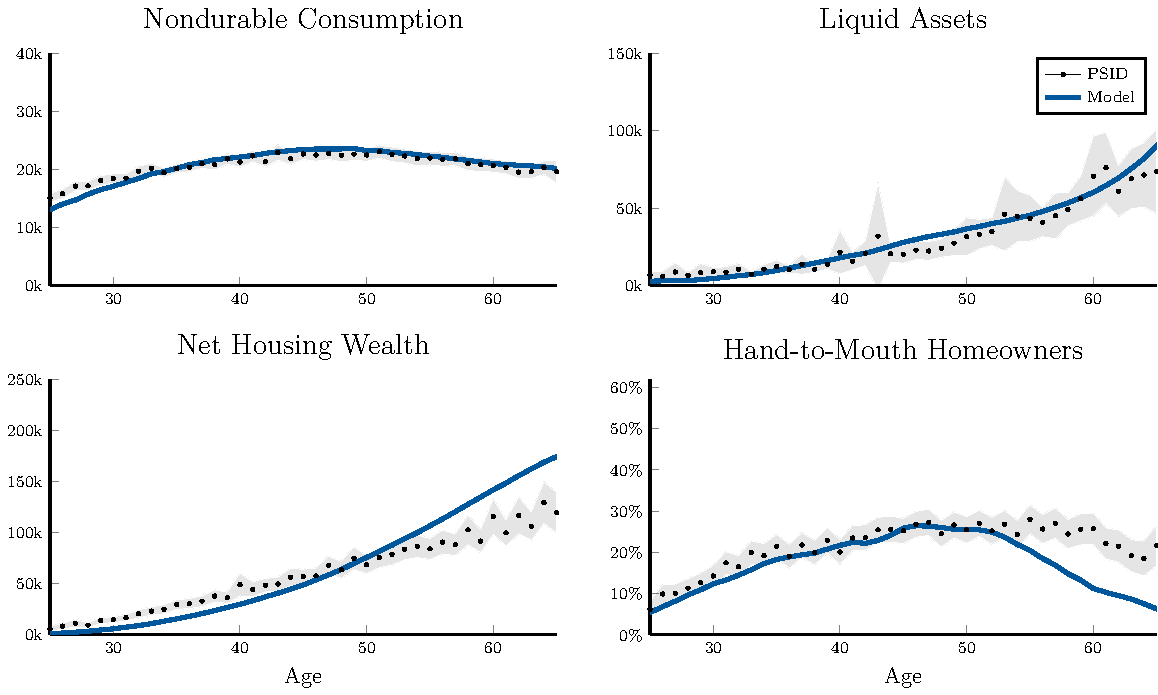
\includegraphics[scale=0.45]{Prezentation_Graphs/TargetedMoments_Temptation}
\end{figure}

Baseline model generates good fit, despite presence of high-return liquid asset

\end{frame}


%---------------------------------------------------------------------%
\begin{frame} {Restricted Model}

\begin{figure}[ht]
\centering
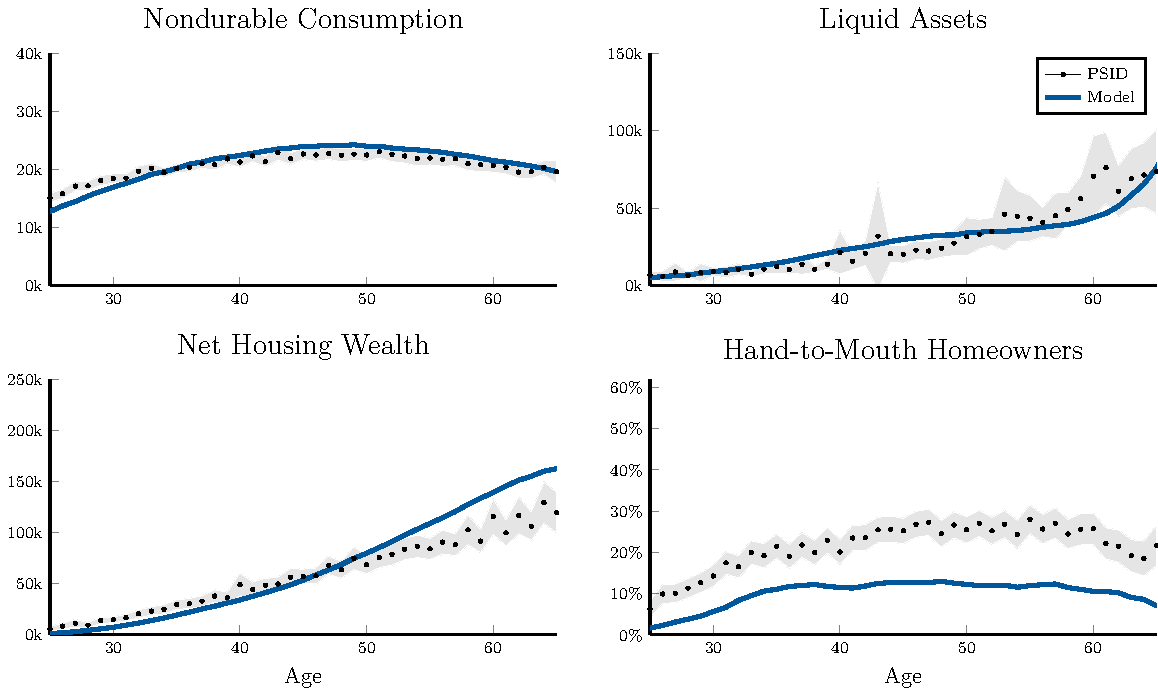
\includegraphics[scale=0.45]{Prezentation_Graphs/TargetedMoments_Standard}
\end{figure}

Restricted model predicts 50\% less hand-to-mouth homeowners

\end{frame}


%---------------------------------------------------------------------%
\begin{frame}{Out-of-Sample Fit}


In addition, the model with temptation \& commitment matches recent empirical evidence showing 
\medskip \medskip 
\begin{enumerate}
	\item The average MPC remains large even in response to large income shocks 
	{\color{gray}\quad (e.g. Fuster, Kaplan, Zafar 2018; Kueng 2018; Fagereng, Holm, Natvik 2021)}
	

	\item Households have a demand for illiquidity {\color{gray}(Beshears et al, 2021)}

	\item Mandatory amortization increases wealth accumulation {\color{gray}(Bernstein and Koudijs, 2021)}
\end{enumerate}

\end{frame}


%%------------------------------------------------------------------------------
\subsection{Implications for Policy}


%---------------------------------------------------------------------%
\begin{frame}{Policy}
\textbf{1. Substantial tax benefits to homeownership in the U.S. }
\begin{itemize} 
\item Mortgage interest tax deduction is \$90 billion/year subsidy (7\% personal income tax)
%	\medskip 
%	\item Seems puzzling in a traditional WH2M framework. Why encourage WH2M behavior?
%	\medskip 
%	\item simply substitute from liquid to illiquid assets
\end{itemize}
\pause

\textbf{2. Growing debate about ``mandatory amortization'' policies}
\begin{itemize}
 
\item Many countries force homeowners to build wealth through mortgage amortization payments
 
\item Concern: May increase WH2M and reduce resilience to income shocks (Svensson, 2019, 2020)

\pause
\end{itemize}

\textbf{We evaluate two opposing views of such illiquid saving incentives}
\begin{itemize}
 
\item May induce portfolio rebalancing from liquid to illiquid assets
 
\item May improve access to commitment, potentially helping HHs accumulate wealth
\end{itemize}

\end{frame}

%---------------------------------------------------------------------%
\begin{frame}{Policy 1: Housing Subsidies}
\begin{figure}[ht]
\centering
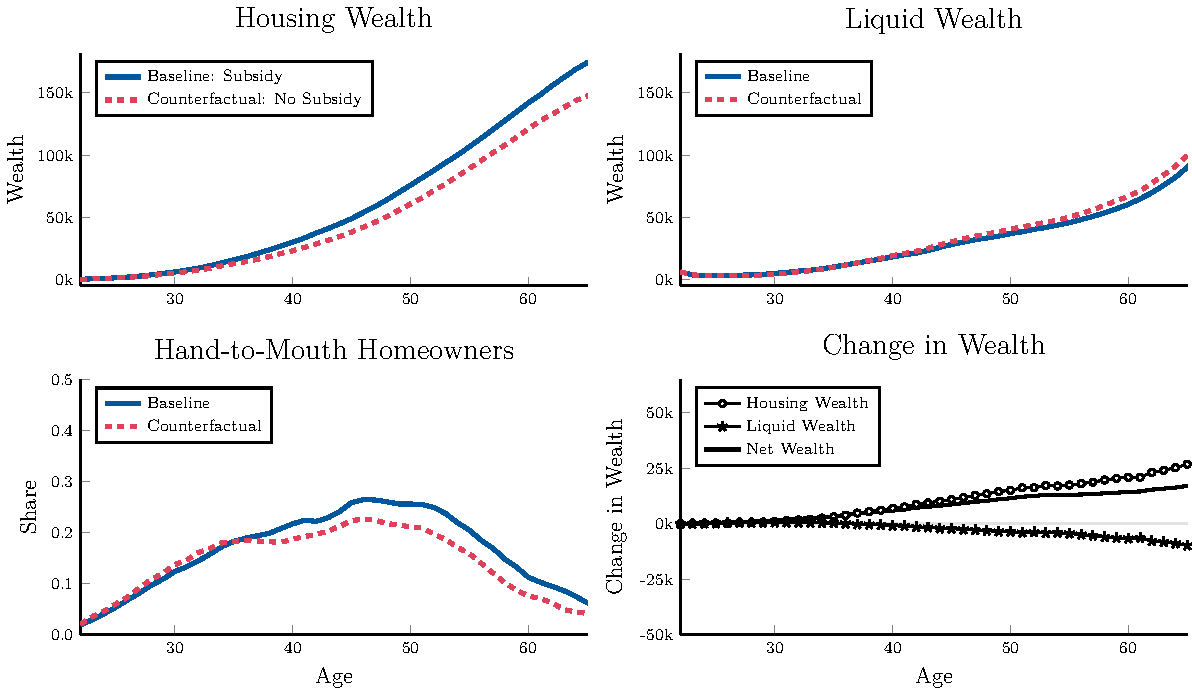
\includegraphics[scale=0.5]{Prezentation_Graphs/HousingSubisdy}
\end{figure}


\end{frame}


%%---------------------------------------------------------------------%
%\begin{frame}{Policy 2: Mandatory Amortization}
%\textbf{Growing debate about ``mandatory amortization'' policies}
%\begin{itemize}
%	\medskip 
%	\item Many countries force homeowners to build wealth through mortgage amortization payments
%	\medskip 
%	\item Concern: May increase WH2M and reduce resilience to income shocks (Svensson, 2019, 2020)
%	\medskip \medskip \medskip 
%	\pause
%\end{itemize}
%
%\textbf{Two opposing views}
%\begin{itemize}
%	\medskip 
%	\item Portfolio rebalancing: from liquid to illiquid
%	\medskip 
%	\item Commitment benefit of housing: may help accumulate wealth
%	\medskip \medskip \medskip 
%	\pause
%\end{itemize}
%
%\textbf{Which effect is more important ? }
%	\medskip 
%	\begin{itemize}
%	\item Model counterfactual: turn off mandatory mortgage amortization
%\end{itemize}
%\end{frame}

%---------------------------------------------------------------------%
\begin{frame}{Policy 2: Mandatory Amortization}
\begin{figure}[ht]
\centering
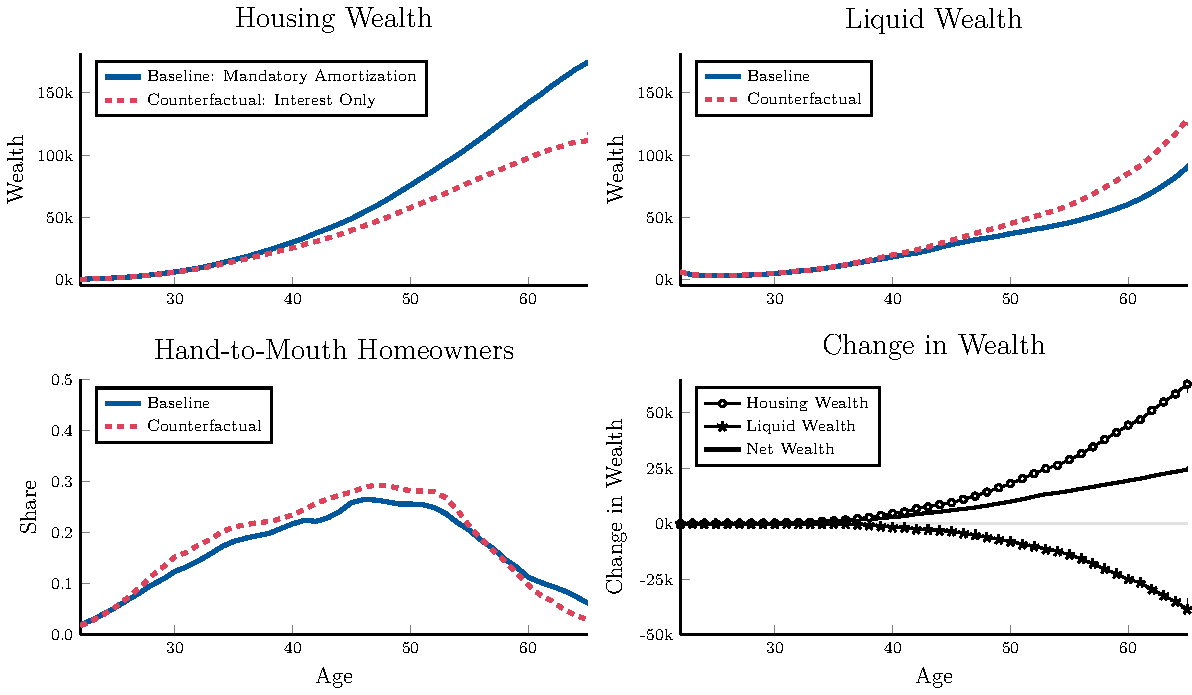
\includegraphics[scale=0.5]{Prezentation_Graphs/MandatoryAmortization}
\end{figure}
\end{frame}





\begin{frame} {Conclusion}


\begin{itemize}

\item Temptation and commitment obtain a good fit of the data
\begin{itemize}
\medskip
\item Large share of WH2M, while relaxing strong assumptions on returns
\medskip
\item Generates good out-of-sample fit of MPCs and recent evidence 

\end{itemize}
%\medskip \medskip \medskip
%\pause
%
%\item Model generates realistic consumption behavior
%\begin{itemize}
%	\medskip
%	\item Large stimulus payments are effective in boosting consumption
%	\medskip
%	\item Model suggests a greater role for targeted fiscal stimulus
%\end{itemize}

\medskip \medskip \medskip
\pause
\item Understanding WH2M behavior has important implications for policy
\begin{itemize}
\medskip
\item Subsidies to commitment can increase overall savings
\medskip
\item Mortgage amortization can boost wealth accumulation
\end{itemize}

\end{itemize}

\end{frame}


\section{Summary}
\begin{frame}{Summary and next week}
\begin{itemize}
	\item <+->\textbf{Today: }Two applications of dynamic programming to
	understand household spending dynamics
	\begin{enumerate}
		\item Macro inattention and its effect on consumption
		\item Temptation to consume for short-term gratification\vfill
	\end{enumerate}
	\item <+->\textbf{Next week: } Learn to extend the workhorse consumption-saving model to include a stationary equilibrium 
	\item <+->\textbf{Homework:}
	\begin{enumerate}
%		\item 
		\item Continue to work on exercises from last week
		\item Start with the model with unemployment from last week, then explore what happens to saving if households have biased beliefs about their job loss probability.*
		\item Read Aiyagari (1994)
	\end{enumerate}
\end{itemize}
\pause
*Biased beliefs = when solving the value function, HHs expect a job loss probability that is different than what happens in the simulation.
\end{frame}
%


%%%%%%%%%%%%%%%  bibliography
%%%%%%%%%%%%%%%%%%%%%%%%%%%%%%%%%%%%%%%%%%%%%%%%%%%%%%%%%%%%%%%%%%%%%%%%%%%%%%%%%%%%%%%%%%%%%%%%%%%%%%%%%%%%%%
\tiny

\beamerdefaultoverlayspecification{<*>}

\begin{frame}[t,allowframebreaks]
\frametitle{References}

%\input econtexBibMake
\write18{if [ ! -f \jobname.bib     ]; then touch \jobname.bib     ; fi}
\write18{if [ ! -f \jobname-Add.bib ]; then touch \jobname-Add.bib ; fi}

\bibliographystyle{econtex}
\bibliography{economics,cAndCwithStickyE-Slides-Add,cAndCwithStickyE-Add}
\end{frame}

\normalsize







\end{document}
